\section{Kalman filter}

The belief can be computed as: 
\[\text{Bel}(x_t|m)=\eta\Pr(z_t|x_t,m)\int\Pr(x_t|u_t,x_{t-1},m)\text{Bel}(x_{t-1}|m)\,dx_{t-1}\]
It can be partially computed using the following two formulas:
\[\begin{cases}
    \bar{\text{Bel}}(x_t|m)=\int\Pr(x_t|u_t,x_{t-1},m)\text{Bel}(x_{t-1}|m)\,dx_{t-1} \\
    \text{Bel}(x_t|m)=\eta\Pr(z_t|x_t,m)\bar{\text{Bel}}(x_t|m)
\end{cases}\]
Note that the variable $\eta$ is also part of an integral.
While it's impossible to compute these integrals in closed form for continuous distributions, it's feasible to do so at least for Gaussian distributions.

\paragraph*{Univariate Gaussian distribution}
The univariate Gaussian distribution, denoted as $X\sim \mathcal{N}(\mu,\sigma^2)$, is described as follows:
\[\Pr(x)=\dfrac{1}{\sqrt{2\pi}\sigma}e^{-\frac{(x-\mu)^2}{2\sigma^2}}\]
\begin{figure}[H]
    \centering
    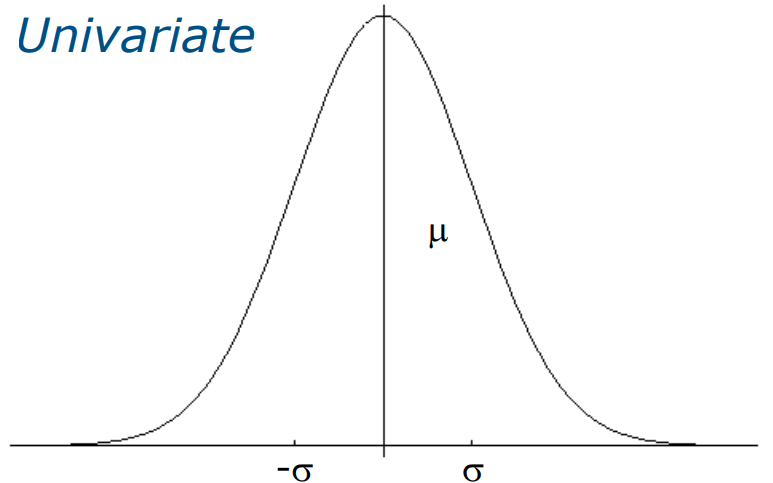
\includegraphics[width=0.6\linewidth]{images/ugd.png}
    \caption{Univariate Gaussian distribution}
\end{figure}
Given an univariate Gaussian distribution $X\sim \mathcal{N}(\mu,\sigma^2)$, the distribution $Y=aX+b$ is still Gaussian and is defined as:
\[Y\sim \mathcal{N}(a\mu+b,a^2\sigma^2)\]
Given two univariate Gaussian distributions $X_1\sim\mathcal{N}(\mu_1,\sigma_1^2)$ and $X_2\sim\mathcal{N}(\mu_2,\sigma_2^2)$, the product of these distributions is:
\[\Pr(X_1)\cdot\Pr(X_2)\sim\mathcal{N}\left(\dfrac{\sigma_2^2}{\sigma_1^2+\sigma_2^2}\mu_1+\dfrac{\sigma_1^2}{\sigma_1^2+\sigma_2^2}\mu_2,\dfrac{1}{\frac{1}{\sigma_1^2}+\frac{1}{\sigma_2^2}}\right)\]

\paragraph*{Multivariate Gaussian distribution}
The multivariate Gaussian distribution, denoted as $X\sim \mathcal{N}(\boldsymbol{\mu},\mathbf{\Sigma})$, is described as follows:
\[\Pr(\mathbf{x})=\dfrac{1}{\sqrt{(2\pi)^d\left\lvert \mathbf{\Sigma} \right\rvert }}e^{-\frac{1}{2}(\mathbf{x}-\boldsymbol{\mu})\mathbf{\Sigma}^{-1}(\mathbf{x}-\boldsymbol{\mu})^T}\]
\begin{figure}[H]
    \centering
    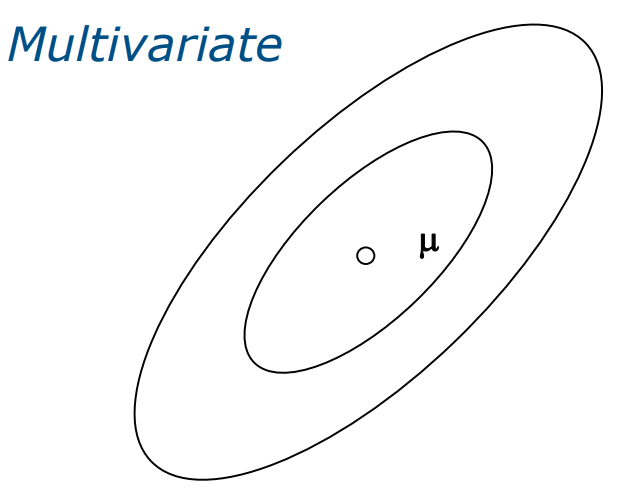
\includegraphics[width=0.6\linewidth]{images/mgd.png}
    \caption{Multivariate Gaussian distribution}
\end{figure}
Given a multivariate Gaussian distribution $X\sim \mathcal{N}(\boldsymbol{\mu},\mathbf{\Sigma})$, the distribution $Y=\mathbf{A}X+\mathbf{B}$ is still Gaussian and is defined as:
\[Y\sim \mathcal{N}(\mathbf{A\mu}+\mathbf{B},\mathbf{A\Sigma A}^T)\]
Given two multivariate Gaussian distributions $X_1\sim\mathcal{N}(\boldsymbol{\mu}_1,\mathbf{\Sigma}_1)$ and $X_2\sim\mathcal{N}(\boldsymbol{\mu}_2,\mathbf{\Sigma}_2)$, the product between these distributions is:
\[\Pr(X_1)\cdot\Pr(X_2)\sim\mathcal{N}\left(\dfrac{\mathbf{\Sigma}_2}{\mathbf{\Sigma}_1+\mathbf{\Sigma}_2}\boldsymbol{\mu}_1+\dfrac{\mathbf{\Sigma}_1}{\mathbf{\Sigma}_1+\mathbf{\Sigma}_2}\boldsymbol{\mu}_2,\dfrac{1}{\frac{1}{\mathbf{\Sigma}_1}+\frac{1}{\mathbf{\Sigma}_2}}\right)\]

\subsection{Discrete time Kalman filter}
Consider the scenario depicted below, where $z$ represents observations, $x$ denotes position, and $u$ signifies the action performed:
\begin{figure}[H]
    \centering
    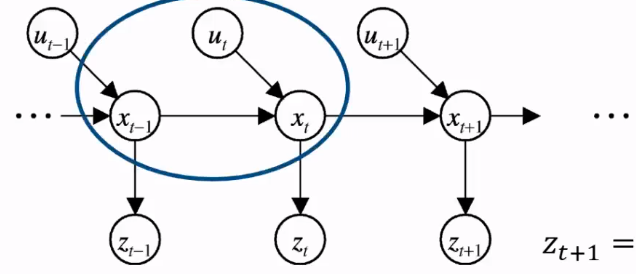
\includegraphics[width=0.75\linewidth]{images/kal.png}
\end{figure}
Let's define the observation as a linear function of the position:
\[z_t=\mathbf{C}_tx_t+\delta_t\]
Here, $C_t$ is a $k\times n$ matrix mapping the state $x_t$ to observation $z_t$, and $\delta_t$ is a random variable representing independent and normally distributed process and measurement noise, with covariance $Q_t$

Similarly, we can model the position of the robot (motion model) as:
\[x_t=\mathbf{A}_tx_{t-1}+\mathbf{B}_tu_t+\varepsilon_t\]
Here, $A_t$ is an $n\times n$ matrix describing state evolution from time $t-1$ to $t$ without controls or noise, $B_t$ is an $n\times l$ matrix illustrating how control $u_t$ affects the state from time $t-1$ to $t$, and $\varepsilon_t$ is a random variable representing independent and normally distributed process and measurement noise, with covariance $R_t$. 

The initial belief is normally distributed:
\[\text{Bel}(x_0)=\mathcal{N}(\boldsymbol{\mu}_0,\mathbf{\Sigma}_0)\]

We assume that observations are linear functions of the state, with additive noise. 
Thus, the probability of having a certain observation becomes:
\[\Pr(z_t|x_t)=\mathcal{N}(z_t;\mathbf{C}_tx_t,\mathbf{Q}_t)\]
Similarly, we assume that states are linear functions of the previous state and control, with additive noise. 
Consequently, the probability of being in a certain state becomes:
\[\Pr(x_t|u_t,x_{t-1})=\mathcal{N}(x_t;\mathbf{A}_tx_{t-1}+\mathbf{B}_tu_t,\mathbf{R}_t)\]

\paragraph*{Closed form prediction}
With these assumptions, we can predict the position as follows:
\begin{align*}
    \bar{\text{Bel}}(x_t)   &=\int\Pr(x_t|u_t,x_{t-1})\cdot\text{Bel}(x_{t-1})\,dx_{t-1} \\
                            &=\int\mathcal{N}(x_t;\mathbf{A}_tx_{t-1}+\mathbf{B}_tu_t,\mathbf{R}_t)\cdot\mathcal{N}(z_t;\mathbf{C}_tx_t,\mathbf{Q}_t)\,dx_{t-1} \\
                            &=\eta\int e^{-\frac{1}{2}(x_t-\mathbf{A}_tx_{t-1}-\mathbf{B}_tu_t)\mathbf{R}_t^{-1}(x_t-\mathbf{A}_tx_{t-1}-\mathbf{B}_tu_t)^T}\cdot e^{-\frac{1}{2}(x_{t-1}-\boldsymbol{\mu}_{t-1})\mathbf{\Sigma}_{t-1}^{-1}(x_{t-1}-\boldsymbol{\mu}_{t-1})^T}\,dx_{t-1}
\end{align*}
In the end, the closed-form prediction step is equal to:
\[\bar{\text{Bel}}(x_t)=\begin{cases}
    \bar{\boldsymbol{\mu}}_t=\mathbf{A}_t\boldsymbol{\mu}_{t-1}+\mathbf{B}_tu_t \\
    \bar{\mathbf{\Sigma}}_t=\mathbf{A}_t\mathbf{\Sigma}_{t-1}\mathbf{A}_t^T+\mathbf{R}_t
\end{cases}\]

\paragraph*{Closed form correction}
With these assumptions, we can correct the position as follows:
\begin{align*}
    \text{Bel}(x_t) &=\eta\Pr(z_t|x_t)\cdot\bar{\text{Bel}}(x_t) \\
                    &=\eta\mathcal{N}(z_t;\mathbf{C}_tx_t,\mathbf{Q}_t)\mathcal{N}(x_t;\bar{\boldsymbol{\mu}}_t,\bar{\boldsymbol{\Sigma}}_t) \\
                    &=\eta\int e^{-\frac{1}{2}(z_t-\mathbf{C}_tx_t)\mathbf{Q}_t^{-1}(z_t-\mathbf{C}_tx_t)^T}\cdot e^{-\frac{1}{2}(x_t-\bar{\boldsymbol{\mu}}_t)  \bar{\mathbf{\Sigma}}_t^{-1}   (x_t-\bar{\boldsymbol{\mu}}_t)^T}\,dx_{t-1}
\end{align*}
In the end, the closed-form update step is equal to:
\[\text{Bel}(x_t)=\begin{cases}
    \mathbf{K}_t=\bar{\mathbf{\Sigma}}_t\mathbf{C}_t^T\left(\mathbf{C}_t\bar{\mathbf{\Sigma}}_t\mathbf{C}_t^T+\mathbf{Q}_t\right)^{-1} \\
    \boldsymbol{\mu}_t=\bar{\boldsymbol{\mu}}_t+\mathbf{K}_t(z_t-\mathbf{C}_t\bar{\boldsymbol{\mu}}_t) \\
    \mathbf{\Sigma}_t=(I-\mathbf{K}_t\mathbf{C}_t)\bar{\mathbf{\Sigma}}_t
\end{cases}\]

\paragraph*{Algorithm} 
With these steps, we can finally construct the Kalman algorithm:
\begin{algorithm}[H]
    \caption{Kalman filter algorithm}
        \begin{algorithmic}[1]
            \State{$\bar{\boldsymbol{\mu}}_t=\mathbf{A}_t\boldsymbol{\mu}_{t-1}+\mathbf{B}_tu_t$} \Comment{Prediction step}
            \State{$\bar{\mathbf{\Sigma}}_t=\mathbf{A}_t\mathbf{\Sigma}_{t-1}\mathbf{A}_t^T+\mathbf{R}_t$} 
            \State{$\mathbf{K}_t=\bar{\mathbf{\Sigma}}_t\mathbf{C}_t^T\left(\mathbf{C}_t\bar{\mathbf{\Sigma}}_t\mathbf{C}_t^T+\mathbf{Q}_t\right)^{-1}$}  \Comment{Correction step}
            \State{$\boldsymbol{\mu}_t=\bar{\boldsymbol{\mu}}_t+\mathbf{K}_t(z_t-\mathbf{C}_t\bar{\boldsymbol{\mu}}_t)$}
            \State{$\mathbf{\Sigma}_t=(I-\mathbf{K}_t\mathbf{C}_t)\bar{\mathbf{\Sigma}}_t$} 
            \State\Return{$\boldsymbol{\mu}_t$,$\mathbf{\Sigma}_t$}
        \end{algorithmic}
\end{algorithm}
The complexity is polynomial in measurement dimensionality $k$ and state dimensionality $n$: $\mathcal{O}(k^{2.376} + n^2)$.
It is optimal for linear Gaussian systems.

However, most robotics systems are nonlinear, and the Kalman filter represents unimodal distributions, limiting its applicability in such cases.

\subsection{Extended Kalman filter}
In linear systems, Gaussian noise is assumed to follow:
\[\begin{cases}
    x_t=\mathbf{A}_tx_{t-1}+\mathbf{B}_tu(t)+\varepsilon_t \\
    z_t=\mathbf{C}_tx_t+\delta_t
\end{cases}\]
However, in non-linear systems, Gaussian noise is distributed as:
\[\begin{cases}
    x_t=g(u_t,x_{t-1}) \\
    z_t=h(x_t)
\end{cases}\]
Here, $g(\cdot)$ and $h(\cdot)$ are nonlinear functions. 

\paragraph*{Prediction step}
In the case of nonlinear functions, the prediction is computed as:
\begin{align*}
    g(u_t,x_{t-1})  &\approx g(u_t,\boldsymbol{\mu}_{t-1})+\dfrac{\partial g(u_t,\boldsymbol{\mu}_{t-1})}{\partial x_{t-1}} (x_{t-1}-\boldsymbol{\mu}_{t-1}) \\
                    &\approx g(u_t,\boldsymbol{\mu}_{t-1})+\mathbf{G}_t(x_{t-1}-\boldsymbol{\mu}_{t-1})
\end{align*} 
Here, $\mathbf{G}_t$ represents the Jacobian matrix of $g(\cdot)$ evaluated at $\left(\boldsymbol{\mu}_{t-1},u(t)\right)$. 

\paragraph*{Correction step}
In case of nonlinear functions we have that the correction is computed as: 
\begin{align*}
    h(x_t)  &\approx h(\bar{\boldsymbol{\mu}}_t)+\dfrac{\partial h(\bar{\boldsymbol{\mu}}_t)}{\partial x_t}(x_t-\bar{\boldsymbol{\mu}}_t) \\
            &\approx h(\bar{\boldsymbol{\mu}}_t)+\mathbf{H}_t(x_t-\bar{\boldsymbol{\mu}}_t)
\end{align*} 
Here, $\mathbf{H}_t$ represents the Jacobian matrix of $h(\cdot)$ evaluated at $\bar{\boldsymbol{\mu}}_t$. 

\paragraph*{Algorithm}
With these steps, we can finally construct the Extended Kalman Filter algorithm:
\begin{algorithm}[H]
    \caption{Extended Kalman filter algorithm}
        \begin{algorithmic}[1]
            \State{$\bar{\boldsymbol{\mu}}_t=g(u_t,\boldsymbol{\mu}_{t-1})$} \Comment{Prediction step}
            \State{$\bar{\mathbf{\Sigma}}_t=\mathbf{G}_t\mathbf{\Sigma}_{t-1}\mathbf{G}_t^T+\mathbf{R}_t$} 
            \State{$\mathbf{K}_t=\bar{\mathbf{\Sigma}}_t\mathbf{H}_t^T\left(\mathbf{H}_t\bar{\mathbf{\Sigma}}_t\mathbf{H}_t^T+\mathbf{Q}_t\right)^{-1}$}  \Comment{Correction step}
            \State{$\boldsymbol{\mu}_t=\bar{\boldsymbol{\mu}}_t+\mathbf{K}_t(z_t-h(\bar{\boldsymbol{\mu}}_t))$}
            \State{$\mathbf{\Sigma}_t=(I-\mathbf{K}_t\mathbf{H}_t)\bar{\mathbf{\Sigma}}_t$} 
            \State\Return{$\boldsymbol{\mu}_t$,$\mathbf{\Sigma}_t$}
        \end{algorithmic}
\end{algorithm}
Here, $\mathbf{G}_t=\frac{\partial g(u_t,\boldsymbol{\mu}_{t-1})}{\partial x_{t-1}}$, and $\mathbf{H}_t=\frac{\partial h(\bar{\boldsymbol{\mu}}_t)}{\partial x_t}$. 
Extended Kalman Filter indeed exhibits polynomial complexity in measurement dimension $k$ and state dimension $n$, typically $\mathcal{O}(k^{2.376} + n^2)$. 
However, it's not optimal and can diverge if nonlinearities are significant. 
Despite its shortcomings, the Extended Kalman Filter often performs well even when some assumptions are violated.

As alternatives, methods like the Unscented Kalman Transform are employed, offering more robustness in handling nonlinearity and uncertainties.